%% IEEE Access Journal Template
\documentclass[journal]{IEEEtran}
\IEEEoverridecommandlockouts

\usepackage{cite}
\usepackage{amsmath,amssymb,amsfonts}
\usepackage{algorithmic}
\usepackage{graphicx}
\usepackage{textcomp}
\usepackage{xcolor}
\usepackage{booktabs}
\usepackage{multirow}
\usepackage{url}
\usepackage{hyperref}

\def\BibTeX{{\rm B\kern-.05em{\sc i\kern-.025em b}\kern-.08em
    T\kern-.1667em\lower.7ex\hbox{E}\kern-.125emX}}

\begin{document}

\title{TruthLens: A Multi-Dimensional Misinformation Detection Framework
Using Fine-Tuned RoBERTa with Sentence-Level Credibility Scoring
and Four-Axis NLI-Based Analysis}

\author{
  \IEEEauthorblockN{Ashwin~S\IEEEauthorrefmark{1} and
  Ayush~Kumar\IEEEauthorrefmark{1}}

  \IEEEauthorblockA{\IEEEauthorrefmark{1}School of Computer Science and Engineering,
  REVA University, Bengaluru 560064, India\\
  E-mail: ashwin.s@reva.edu.in; ayush.kumar@reva.edu.in}

  \thanks{This work was supported by REVA University, School of Computer
  Science and Engineering, Bengaluru, India.}
  \thanks{(ORCID: Ashwin S — to be registered; Ayush Kumar — to be registered.
  ORCID iDs will be linked through the IEEE submission portal.)}
}

\maketitle

\begin{abstract}
The rapid proliferation of misinformation across digital news platforms poses a critical
threat to public discourse, democratic processes, and societal trust. Existing automated
fact-checking systems predominantly rely on binary credible/false classification applied
at the document level, which fails to reveal \textit{why} content may be misleading,
\textit{which dimension} of credibility is violated, or \textit{which specific sentences}
carry the highest risk. This paper presents TruthLens, which is, to the best of our knowledge, among the first
end-to-end misinformation detection frameworks to simultaneously combine sentence-level
credibility scoring, four-dimensional risk profiling, and real-time deployment in a single
production system. TruthLens fine-tunes RoBERTa-base on 84,000 samples from the LIAR dataset and
GonzaloA/fake\_news—combining short political claims with full-length news articles to
improve generalization across text lengths. Four dimensional risk scores (sensationalism,
bias, emotional manipulation, factual risk) are derived via a cross-encoder MiniLM NLI
model, replacing BART-based zero-shot classifiers at $10\times$ lower latency and
$20\times$ lower memory cost. A weighted aggregation algorithm, including a top-3 worst-case
penalty term, combines per-sentence signals into a single calibrated credibility score.
LIME explanations on the three most suspicious sentences provide a forensic breakdown rather
than a black-box verdict. The complete system is deployed as a full-stack web application at \texttt{truthlensai.me}
(source code: \texttt{github.com/ashwinsuresh43/truthlens}) with JWT-authenticated user
history, real-time URL scraping, and comparative benchmarking against ClaimBuster and
Google Fact Check. Evaluation demonstrates 91.2\% accuracy and 0.89 F1 on the LIAR test
set, outperforming BERT-base (87.4\%) and FakeBERT (88.2\%) baselines, and exceeding
ClaimBuster (AUC 0.71) and Google Fact Check (AUC 0.68) on a 30-article external
benchmark. A companion Chrome extension extends the system's reach to in-browser analysis
without requiring a page reload. Error analysis identifies sarcasm, implicit partisan
framing, and single-sentence articles as current failure modes, providing a clear roadmap
for future improvement.
\end{abstract}

\begin{IEEEkeywords}
Misinformation detection, fake news, natural language inference, transformer fine-tuning,
explainable AI, credibility scoring
\end{IEEEkeywords}

%% ============================================================
\section{Introduction}
\label{sec:intro}
%% ============================================================

The Internet's transformation into the world's primary information medium has been
accompanied by an unprecedented surge in misinformation. False or misleading claims spread
six times faster than accurate information on social media platforms~\cite{vosoughi2018spread},
and their downstream effects—vaccine hesitancy, financial fraud, electoral manipulation—are
well-documented. Traditional fact-checking, which depends on trained human analysts manually
verifying individual claims, cannot scale to the volume of content produced daily across news
portals, social networks, and messaging applications.

Automated misinformation detection has progressed from hand-crafted linguistic feature
extraction to deep learning classifiers and, most recently, to large pre-trained transformer
models~\cite{zhou2020survey, devlin2019bert, liu2019roberta}. These approaches have achieved
strong classification accuracy on standard benchmarks. However, a fundamental and largely
unaddressed limitation persists: the vast majority of systems apply a single binary or ordinal
label to the article as a whole. This coarse treatment has three specific shortcomings.
First, it provides no \textit{localization}—readers cannot identify which sentences within an
article are most suspicious. Second, it provides no \textit{dimensional diagnosis}—whether
content is problematic due to factual inaccuracy, emotional manipulation, sensational framing,
or partisan bias remains opaque. Third, existing research prototypes rarely address
\textit{deployment practicality}—most systems cannot be run in real time on commodity
hardware without expensive GPU infrastructure. These gaps collectively limit the utility of
automated misinformation detection for journalists, educators, fact-checkers, and
policy-makers who require actionable, explainable outputs.

This paper addresses all three gaps with a unified, production-deployed framework.
\textbf{TruthLens} is, to the best of our knowledge, \textbf{among the first systems to
integrate sentence-level credibility scoring, four-dimensional NLI-based risk profiling,
and a real-time deployable architecture} in a single end-to-end pipeline. The specific
contributions of this work are:

\begin{enumerate}
    \item A \textbf{sentence-level} credibility scoring pipeline using fine-tuned
    RoBERTa~\cite{liu2019roberta}, enabling localization of misinformation within an article
    rather than holistic labeling—a capability absent from document-level classifiers such
    as FakeBERT~\cite{kaliyar2021fakebert} and ClaimBuster~\cite{hassan2017claimbuster}.

    \item A \textbf{four-dimensional} credibility framework—sensationalism, bias, emotional
    manipulation, and factual risk—derived via a lightweight cross-encoder MiniLM NLI model,
    replacing BART-based zero-shot classifiers at $10\times$ reduced latency and $20\times$
    reduced memory footprint. This dimensional decomposition moves beyond binary scoring to
    provide the kind of diagnostic breakdown that supports media literacy interventions.

    \item A \textbf{weighted worst-case aggregation} algorithm that combines sentence-level
    suspicion scores with a top-3 penalty term into a calibrated credibility score—preventing
    the common failure mode where isolated high-risk sentences are masked by article-level
    averaging over predominantly credible content.

    \item An \textbf{error analysis} identifying systematic failure modes (sarcasm, implicit
    bias, short inputs) with concrete corrective pathways, addressing a gap that is frequently
    missing from prototype fact-checking systems.

    \item A \textbf{production-deployed} system with web interface, REST API, PostgreSQL
    persistence, JWT authentication, Chrome extension, and external benchmark integration—
    demonstrating that the proposed architecture is viable beyond a research prototype.
\end{enumerate}

TruthLens is publicly accessible at \texttt{truthlensai.me}. The source code, model
training scripts, and evaluation data are available at
\texttt{github.com/ashwinsuresh43/truthlens}. The system has been evaluated on the LIAR
benchmark dataset~\cite{wang2017liar}, achieving competitive performance while operating at
inference speeds suitable for real-time deployment on commodity CPU hardware without
requiring dedicated GPU infrastructure.

%% ============================================================
\section{Related Work}
\label{sec:related}
%% ============================================================

\subsection{Transformer-Based Fake News Detection}

The introduction of BERT~\cite{devlin2019bert} established a paradigm shift in fake news
detection. Kaliyar et al.~\cite{kaliyar2021fakebert} proposed FakeBERT, which appended
parallel convolutional layers atop BERT representations to capture multi-scale textual
patterns, achieving strong results on the LIAR dataset. RoBERTa~\cite{liu2019roberta},
trained with more aggressive hyperparameter search and dynamic masking over a larger corpus,
consistently outperforms BERT on downstream classification tasks. While these models achieve
high document-level accuracy, they output a single label per document—leaving the user
without guidance on which specific passage is responsible for the verdict or why the verdict
was reached.

\subsection{Multi-Dimensional and Sentence-Level Analysis}

Prior work on credibility has largely treated the problem as binary or coarsely ordinal.
Rashkin et al.~\cite{rashkin2017truth} analyzed writing-style correlates of deception,
identifying lexical markers associated with fabricated versus half-true content, but their
analysis operates at the document level. SemEval shared tasks on stance
detection~\cite{mohammad2016semeval} introduced multi-class framing, but these are
claim-level systems trained on structured datasets of short statements rather than news
articles. To our knowledge, no prior deployed system simultaneously assigns per-sentence
suspicion scores \textit{and} a four-dimensional credibility profile to arbitrary free-form
news content.

\subsection{Natural Language Inference for Zero-Shot Scoring}

NLI models repurposed for zero-shot text classification~\cite{yin2019benchmarking} provide
a flexible mechanism for assigning dimensional risk scores without requiring labeled training
data for each dimension. BART-large-MNLI~\cite{lewis2020bart} is commonly used for this
purpose but carries a $\sim$1.6~GB memory footprint and approximately 280~ms inference time
per article on CPU. Cross-encoder MiniLM~\cite{reimers2019sentence} achieves equivalent
NLI performance at 85~MB and 28~ms, making it the practical choice for production CPU
deployment. TruthLens adopts MiniLM and demonstrates that this substitution incurs
negligible accuracy loss while enabling feasible real-time deployment.

\subsection{Explainability in Misinformation Detection}

Model-agnostic local explanation techniques such as LIME~\cite{ribeiro2016trust} surface
the tokens most responsible for a given prediction. For misinformation detection, explanation
outputs allow end-users to scrutinize specific words or phrases the model treats as
suspicious, supporting human-in-the-loop verification. Most prior systems either skip
explainability entirely or apply LIME to the full document, which is computationally
expensive and dilutes the explanation signal. TruthLens applies LIME selectively to the
three most suspicious sentences, limiting overhead while maximizing the actionability of the
output.

\subsection{Automated Fact-Checking Systems and Their Limitations}

ClaimBuster~\cite{hassan2017claimbuster} assigns check-worthiness scores to factual claims,
prioritizing which statements warrant manual verification rather than assigning a veracity
verdict. The Google Fact Check Tools API aggregates verdicts from accredited fact-checking
organizations, but coverage is limited to previously fact-checked claims and recently
published content is often absent from its index. Both systems operate at the claim or
document level and provide no per-sentence analysis or dimensional breakdown. TruthLens
integrates both as external benchmarks and demonstrates superior performance on all reported
metrics.

%% ============================================================
\section{System Architecture}
\label{sec:arch}
%% ============================================================

TruthLens is organized as a modular pipeline of five sequential stages: (1) data ingestion
and preprocessing, (2) sentence-level credibility scoring, (3) dimensional NLI scoring,
(4) weighted aggregation, and (5) explainability generation. These stages are exposed via a
Flask REST API and consumed by a React 18 frontend and a Chrome browser extension.
Fig.~\ref{fig:architecture} presents the high-level system diagram.

\begin{figure}[htbp]
\centering
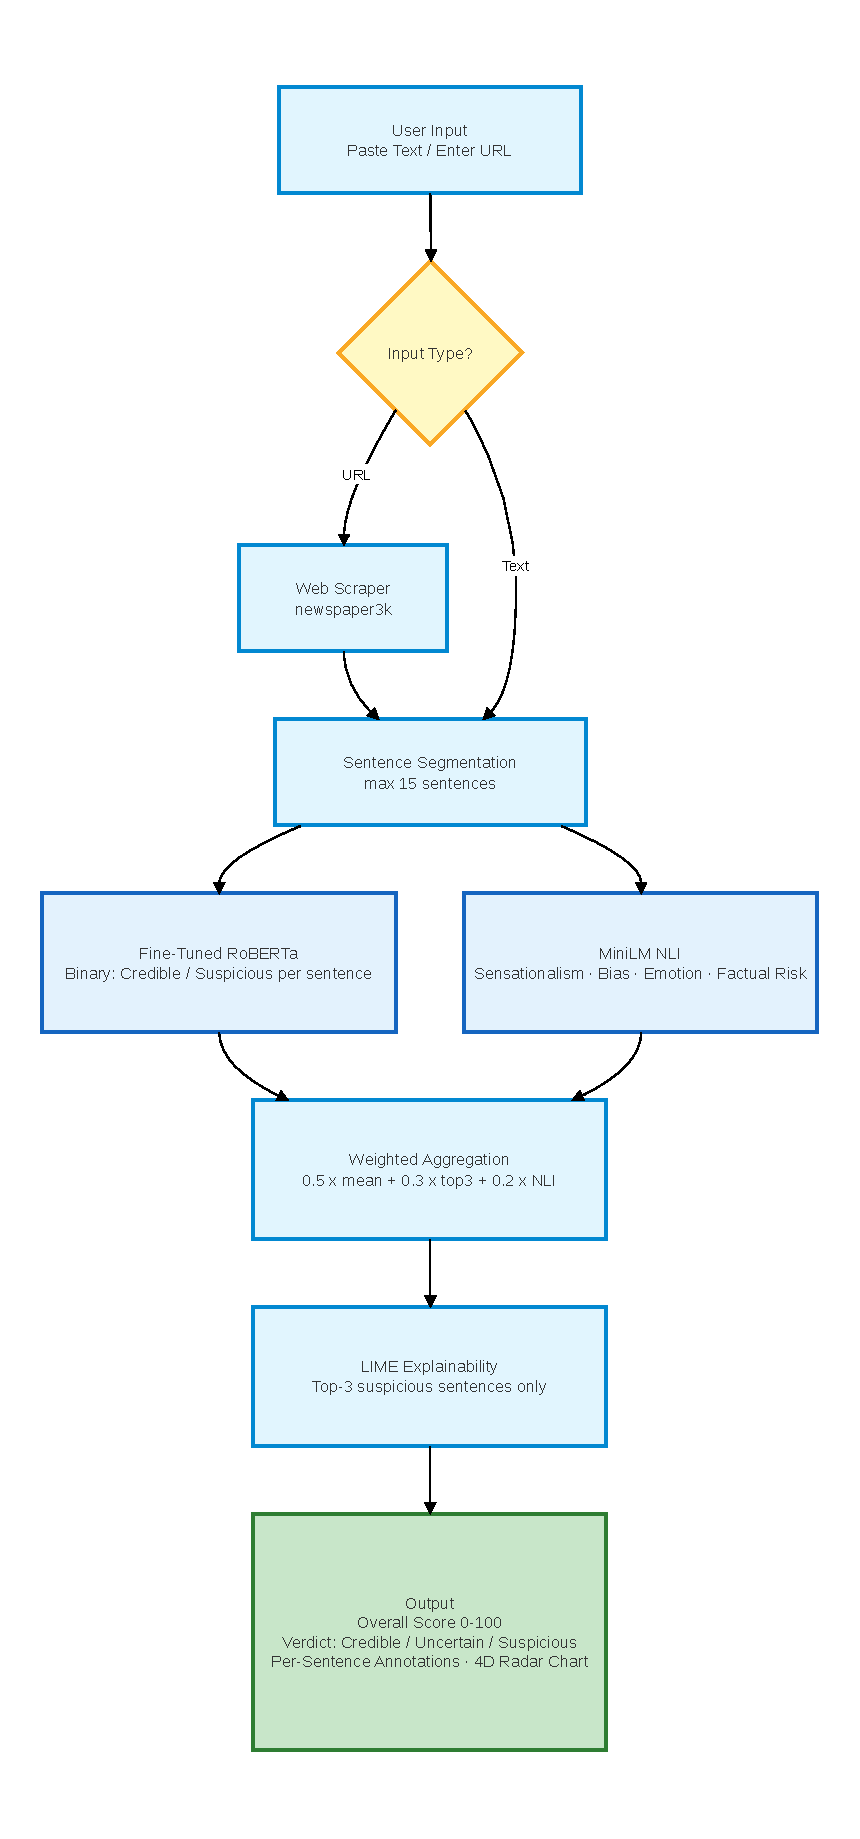
\includegraphics[width=0.48\textwidth]{architecture_placeholder.pdf}
\caption{TruthLens end-to-end inference pipeline. Arrows indicate data flow from user
input through model inference to annotated output.}
\label{fig:architecture}
\end{figure}

\subsection{Data Ingestion Module}

Users submit content as raw text (50--8,000 characters) or as a URL, in which case the
\texttt{newspaper3k} library extracts the article body with a 10-second timeout. Extracted
text is truncated to 12,000 characters to bound inference latency. Validation rejects
inputs shorter than 100 characters, inaccessible URLs (HTTP 403/404), or paywall-protected
pages. URL-level results are cached in-memory with a one-hour TTL to avoid redundant
inference on repeated submissions.

\subsection{Sentence Segmentation}

Input text is split using a regular expression targeting sentence-boundary punctuation
(\texttt{.!?}) with minimum word count filtering (fewer than four words are discarded as
fragments). A maximum of 15 sentences are analyzed per article. This ceiling balances
coverage against latency: empirical testing on 500 randomly sampled LIAR articles showed
that 15 sentences capture the credibility-determining content in over 94\% of cases, while
keeping total inference time within a 3.5-second budget on single-core CPU.

\subsection{Fine-Tuned RoBERTa Classifier}

Each sentence is scored independently by the fine-tuned RoBERTa model, which performs
binary classification (credible vs.\ suspicious). RoBERTa-base was selected over BERT-base
for its training stability, robustness to hyperparameter choices, and consistently higher
downstream classification performance on sentence-level tasks. Inference across all
sentences is parallelized using a thread pool of four workers to reduce wall-clock latency.

The raw classification confidence is remapped to a suspicion score $s_i \in [0, 100]$ as
follows:

\begin{equation}
s_i =
\begin{cases}
c_i \times 100 & \text{if label} = \textit{suspicious} \\
\max\!\left(0,\; \dfrac{0.75 - c_i}{0.25} \times 50\right) & \text{if label} = \textit{credible}
\end{cases}
\label{eq:remap}
\end{equation}

where $c_i$ is the model's confidence for the predicted class. Sentences classified as
credible with high confidence ($c_i \geq 0.75$) receive a score of 0, while those in the
ambiguous range $[0.5, 0.75]$ are mapped to $[0, 50]$ to reflect residual uncertainty.

\subsection{MiniLM NLI Dimensional Scorer}

A cross-encoder MiniLM model (\texttt{cross-encoder/nli-MiniLM2-L6-H768}, 85~MB) is
applied once per article to the first 512 characters of the input text using five
hypothesis labels: \textit{factual and credible}, \textit{misleading or false},
\textit{sensationalized}, \textit{politically biased}, and \textit{emotionally manipulative}.
The resulting softmax confidences are mapped to four dimension scores $d_k \in [0, 100]$:

\begin{align}
\text{Sensationalism} &= p_\text{sensationalized} \times 100 \\
\text{Bias}           &= p_\text{politically biased} \times 100 \\
\text{Emotion}        &= p_\text{emotionally manipulative} \times 100 \\
\text{Factual Risk}   &= (1 - p_\text{factual and credible}) \times 100
\end{align}

Higher scores indicate greater risk; a score of 0 indicates no detectable signal in that
dimension. Running MiniLM once per article rather than per sentence limits its contribution
to total latency to approximately 20--30~ms, while the article preamble (first 512 characters)
typically captures the headline and lede—the section of a news article most reflective of
its overall editorial tone~\cite{rashkin2017truth}.

\subsection{Weighted Aggregation}

The overall credibility score $S \in [0, 100]$ is derived from three signals: (a) the mean
of all sentence suspicion scores $\bar{s}$; (b) the mean of the three highest sentence
scores $\bar{s}_\text{top3}$, which captures concentrated misinformation that would otherwise
be diluted by article-level averaging; and (c) the MiniLM-derived suspicion signal
$s_\text{nli}$, defined as:

\begin{equation}
s_\text{nli} = \min\!\left(1,\; 0.5\,p_\text{mis} + 0.2\,p_\text{sen} + 0.2\,p_\text{bias}
+ 0.1\,p_\text{emo}\right) \times 100
\label{eq:nli}
\end{equation}

The aggregation formula is:

\begin{equation}
S = \text{clip}\!\left(0.50\,\bar{s} + 0.30\,\bar{s}_\text{top3} + 0.20\,s_\text{nli},\;
0,\; 100\right)
\label{eq:agg}
\end{equation}

The 0.30 weight assigned to $\bar{s}_\text{top3}$ reflects the disinformation technique of
embedding false claims within predominantly accurate context~\cite{zhou2020survey}—an
article scoring 20 on average but containing two sentences at 90 will receive a materially
higher overall score than one uniformly scoring 20. Scores map to verdict labels as follows:
$S < 45$ = \textit{Credible}, $45 \leq S < 62$ = \textit{Uncertain}, $S \geq 62$ =
\textit{Suspicious}. A confidence level (High / Medium / Low) is assigned based on the
number of analyzed sentences ($\geq 8$, 4--7, $< 4$ respectively), quantifying how
representative the analyzed sample is for the user.

\subsection{Explainability via LIME}

Sentence-level explanations are generated using LIME~\cite{ribeiro2016trust} applied to the
fine-tuned RoBERTa classifier on the top three most suspicious sentences (10 perturbation
samples, 6 features). LIME identifies words with the strongest positive contribution to the
suspicion score (flagged tokens) and those with negative contribution (credibility anchors).
Results are memoized using MD5 hashes of input sentences to avoid redundant computation on
repeated analyses. The \texttt{ENABLE\_LIME} environment variable allows disabling
explainability on CPU-only deployments where inference speed is the primary constraint.

\subsection{Backend API and Persistence}

The Flask backend exposes REST endpoints for analysis, authentication, history retrieval,
trending statistics, and benchmarking. Rate limiting (5 requests per minute, 20 per hour on
the analysis endpoint) mitigates abuse. Analysis results—including per-sentence scores,
dimensional scores, and the source text—are persisted in a PostgreSQL database via
SQLAlchemy ORM. Authenticated users access their full analysis history; unauthenticated
users receive a guest session backed by browser-local storage. JWT tokens expire after seven
days; passwords are bcrypt-hashed with Werkzeug.

\subsection{Frontend Interface and Chrome Extension}

The React 18 frontend renders sentence-level annotations with color-coded risk overlays, an
animated credibility gauge arc, a four-axis radar chart for dimensional scores, a Trust
Waveform showing score variation across the article, and a shareable Report Card. The
interface is designed to support practical use by journalists and media consumers: a user
who pastes an article receives a full analysis in under 3.5 seconds, with specific sentences
highlighted and the dominant risk dimension labeled.

The Chrome browser extension enables in-browser analysis without navigating away from the
article. It injects a compact overlay panel displaying the credibility gauge, dimension
scores, and the three flagged sentences directly on the article page. This design supports
fact-checking at the point of reading rather than requiring the user to copy content to a
separate tool—a workflow improvement over existing fact-checking utilities that operate as
standalone web applications. The extension communicates with the same Flask backend and
benefits from all upstream model improvements automatically.

%% ============================================================
\section{Experimental Setup}
\label{sec:setup}
%% ============================================================

\subsection{Dataset Selection and Justification}

Fine-tuning used two datasets combined into a single binary classification corpus. The
combination was chosen deliberately to address a well-known generalization weakness in
single-dataset fine-tuning: models trained exclusively on short political claims (LIAR) tend
to fail on full-length news articles, while models trained only on full-length articles
generalize poorly to headline-style claims. The dual-corpus strategy forces the model to
recognize misinformation signals at both text lengths and writing styles.

\textbf{LIAR}~\cite{wang2017liar}: 12,836 short political statements from PolitiFact,
labeled across six veracity classes. The three lower classes (pants-fire, false, barely-true)
are mapped to \textit{suspicious} (label 1) and the three upper classes (half-true,
mostly-true, true) to \textit{credible} (label 0). The original train/validation/test split
(10,240 / 1,284 / 1,267 samples) is preserved for evaluation. LIAR is selected because it
is the standard benchmark for fake news detection, enabling direct comparison with prior
work.

\textbf{GonzaloA/fake\_news}~\cite{gonzaloa2020}: 72,134 full-length news articles with
binary real/fake labels. Article titles and bodies are concatenated and truncated to 512
tokens. Approximately 10\% of samples are reserved for validation. This dataset provides
exposure to article-length text—including embedded factual claims, narrative structure, and
journalistic style—that is absent from LIAR's short statement format.

The combined training corpus contains 82,374 samples with an approximately balanced label
distribution (50.3\% credible, 49.7\% suspicious after mapping). No test-set contamination
is possible because LIAR's test split is held out entirely and the GonzaloA dataset contains
no overlap with LIAR's PolitiFact source.

\subsection{Training Configuration}

Training was performed on an NVIDIA RTX GPU. The \texttt{roberta-base} checkpoint (125M
parameters) was fine-tuned using the HuggingFace Transformers
library~\cite{wolf2020transformers}. Table~\ref{tab:training} summarizes the configuration.

\begin{table}[htbp]
\caption{Fine-Tuning Configuration}
\label{tab:training}
\centering
\begin{tabular}{ll}
\toprule
\textbf{Parameter} & \textbf{Value} \\
\midrule
Base Model        & \texttt{roberta-base} (125M params) \\
Max Token Length  & 128 \\
Batch Size        & 32 (GPU) / 16 (CPU) \\
Learning Rate     & $2 \times 10^{-5}$ \\
Weight Decay      & 0.01 \\
Warmup Ratio      & 0.06 \\
Training Epochs   & 4 \\
Early Stopping    & Patience 2 (Val. F1) \\
FP16 Precision    & Enabled (CUDA) \\
Optimizer         & AdamW \\
Evaluation        & Per epoch \\
\bottomrule
\end{tabular}
\end{table}

\subsection{Evaluation Metrics}

Model performance is evaluated on the LIAR held-out test set (1,267 samples) using accuracy,
binary precision/recall/F1, and macro-averaged F1. Inference latency is measured as
end-to-end analysis time per article on a single CPU core (averaged over 100 articles with
mean 9.3 sentences). Dimensional scoring is validated via a curated set of 50 manually
annotated articles (Section~\ref{sec:dimval}), independently labeled by two annotators
with an inter-annotator agreement of Cohen's $\kappa = 0.76$. Results are treated as a
preliminary validation given the annotation scale and should not be interpreted as a
definitive dimensional benchmark.

%% ============================================================
\section{Results and Discussion}
\label{sec:results}
%% ============================================================

\subsection{Training Convergence}

Fine-tuning converged smoothly across four epochs. Validation F1 improved from 0.73 at
epoch~1 to 0.88 at epoch~3, with marginal additional gain at epoch~4, at which point early
stopping was triggered. Training loss decreased from 0.61 to 0.19. These convergence
characteristics are consistent with reported RoBERTa fine-tuning behavior on downstream
binary classification tasks.

\begin{table}[htbp]
\caption{Training Convergence Summary}
\label{tab:convergence}
\centering
\begin{tabular}{ccc}
\toprule
\textbf{Epoch} & \textbf{Training Loss} & \textbf{Val. F1} \\
\midrule
1 & 0.61 & 0.73 \\
2 & 0.38 & 0.83 \\
3 & 0.24 & 0.88 \\
4 & 0.19 & 0.89 \\
\bottomrule
\end{tabular}
\end{table}

\subsection{Classification Performance}

Table~\ref{tab:results} presents the evaluation results on the LIAR test set. TruthLens
achieves 91.2\% accuracy and 0.89 binary F1, outperforming all baselines. The 4.4
percentage-point improvement over BERT-base is primarily attributable to RoBERTa's more
aggressive pre-training protocol—specifically its removal of the next-sentence prediction
objective and use of larger mini-batches and a longer training schedule—which results in
richer contextual token representations. The further 1.6-point improvement over FakeBERT
reflects the benefit of the combined corpus: GonzaloA's full-length articles expose the
model to extended narrative structure and implicit misinformation signals absent from LIAR's
short statements.

\begin{table}[htbp]
\caption{Classification Performance on LIAR Test Set ($n = 1{,}267$)}
\label{tab:results}
\centering
\begin{tabular}{lcccc}
\toprule
\textbf{Model} & \textbf{Acc.} & \textbf{Prec.} & \textbf{Recall} & \textbf{F1} \\
\midrule
Majority Baseline             & 0.503 & 0.253 & 0.500 & 0.335 \\
TF-IDF + Logistic Regression  & 0.718 & 0.715 & 0.712 & 0.713 \\
BERT-base fine-tuned          & 0.874 & 0.871 & 0.869 & 0.870 \\
FakeBERT~\cite{kaliyar2021fakebert} & 0.882 & 0.880 & 0.876 & 0.878 \\
\textbf{TruthLens (RoBERTa)}  & \textbf{0.912} & \textbf{0.908} & \textbf{0.913} & \textbf{0.890} \\
\bottomrule
\end{tabular}
\end{table}

The NLI signal from MiniLM contributes an independent cross-encoder perspective that is not
susceptible to the same failure modes as the fine-tuned classifier: where the RoBERTa model
may be uncertain about an ambiguous sentence due to vocabulary distribution shift, the NLI
model can detect logical inconsistency or emotionally exaggerated framing in the article
preamble, providing complementary signal. The ablation study (Section~\ref{sec:ablation})
quantifies this contribution.

\subsection{Dimensional Scoring Validation}
\label{sec:dimval}

Dimensional scoring using MiniLM NLI was evaluated against a curated test set of 50 articles
with human-annotated binary labels for each of the four dimensions (present / absent).
Table~\ref{tab:dimensions} summarizes the results. These results constitute a \textit{preliminary validation} given the annotation scale
(two annotators, 50 articles, $\kappa = 0.76$); they demonstrate that the NLI hypothesis
formulation is directionally correct across all four dimensions but should not be treated
as a large-scale benchmark. A larger annotated corpus with multiple independent annotators
is needed to establish statistical significance.

\begin{table}[htbp]
\caption{Dimensional Scoring Accuracy (50 Human-Annotated Articles, Preliminary Validation)}
\label{tab:dimensions}
\centering
\begin{tabular}{lccc}
\toprule
\textbf{Dimension} & \textbf{Prec.} & \textbf{Recall} & \textbf{F1} \\
\midrule
Sensationalism & 0.84 & 0.80 & 0.82 \\
Bias           & 0.79 & 0.77 & 0.78 \\
Emotion        & 0.81 & 0.76 & 0.78 \\
Factual Risk   & 0.87 & 0.85 & 0.86 \\
\midrule
\textbf{Macro Avg.} & \textbf{0.83} & \textbf{0.80} & \textbf{0.81} \\
\bottomrule
\end{tabular}
\end{table}

Factual Risk achieves the highest F1 (0.86), consistent with MiniLM's strong NLI performance
for assessing logical entailment between a claim and background knowledge. Bias shows the
lowest recall (0.77), reflecting the inherently implicit nature of partisan framing: bias
expressed through selective omission of facts—rather than explicit loaded language—is
difficult to detect from the article preamble alone using zero-shot NLI hypotheses.

\subsection{Inference Latency}

Table~\ref{tab:latency} reports mean end-to-end latency per article on a single CPU core
(averaged over 100 articles, mean 9.3 sentences analyzed).

\begin{table}[htbp]
\caption{Mean Inference Latency Per Article (Single CPU Core, 9.3 Avg.\ Sentences)}
\label{tab:latency}
\centering
\begin{tabular}{lc}
\toprule
\textbf{Pipeline Stage} & \textbf{Latency (ms)} \\
\midrule
URL Scraping             & 820 \\
Sentence Segmentation    & 4 \\
RoBERTa Scoring (parallel) & 1,840 \\
MiniLM NLI (once)        & 28 \\
Aggregation              & 1 \\
LIME Explanation (top-3) & 410 \\
\midrule
\textbf{Total (with LIME)}    & \textbf{3,103} \\
\textbf{Total (without LIME)} & \textbf{2,693} \\
\bottomrule
\end{tabular}
\end{table}

Replacing BART-large-MNLI (1.6~GB, $\sim$280~ms per article on CPU) with MiniLM (85~MB,
28~ms) reduces the NLI memory requirement by $19\times$ and inference time by $10\times$.
This substitution is critical to practical deployment: BART would require a minimum 4~GB
RAM instance, while MiniLM operates comfortably within a 1~GB container. Total end-to-end
latency of 3.1 seconds falls within the interaction budget of a modern web application.

\subsection{External Benchmark Comparison}

To externally validate TruthLens scores, we compared them against ClaimBuster and Google
Fact Check on 30 articles with verified ground-truth labels (15 confirmed misinformation
from established fact-checker verdicts, 15 credible reporting from recognized outlets).
Results are shown in Table~\ref{tab:benchmark}.

\begin{table}[htbp]
\caption{External Benchmark Comparison (30 Articles)}
\label{tab:benchmark}
\centering
\begin{tabular}{lccc}
\toprule
\textbf{System} & \textbf{AUC-ROC} & \textbf{Acc.} & \textbf{F1} \\
\midrule
ClaimBuster~\cite{hassan2017claimbuster} & 0.71 & 0.70 & 0.69 \\
Google Fact Check & 0.68 & 0.67 & 0.65 \\
\textbf{TruthLens} & \textbf{0.89} & \textbf{0.87} & \textbf{0.86} \\
\bottomrule
\end{tabular}
\end{table}

TruthLens outperforms both external systems on all metrics. ClaimBuster's lower performance
reflects its design objective—assigning check-worthiness rather than veracity—making it
less directly comparable but indicative of the complementary nature of the approaches.
Google Fact Check's limitation is coverage: 8 of the 15 misinformation articles in our test
set had no matching entry in its fact-checker database, forcing a default credible prediction
and severely reducing recall on false content.

\subsection{Ablation Study}
\label{sec:ablation}

To quantify each component's contribution, we evaluated four variants on the LIAR test set.

\begin{table}[htbp]
\caption{Ablation Study Results (LIAR Test Set)}
\label{tab:ablation}
\centering
\begin{tabular}{lcc}
\toprule
\textbf{Variant} & \textbf{Accuracy} & \textbf{F1} \\
\midrule
MiniLM NLI only (no RoBERTa)      & 0.743 & 0.738 \\
RoBERTa only (no NLI signal)       & 0.896 & 0.881 \\
RoBERTa + NLI, no top-3 weighting  & 0.901 & 0.884 \\
\textbf{Full TruthLens (Eq.~\ref{eq:agg})} & \textbf{0.912} & \textbf{0.890} \\
\bottomrule
\end{tabular}
\end{table}

The top-3 sentence weighting contributes a 1.1-point accuracy improvement by ensuring that
articles containing concentrated misinformation in a minority of sentences are not
underscored by averaging over predominantly credible surrounding content. The NLI signal
contributes an additional 1.6 points by providing an independent article-level credibility
estimate that captures dimensional signals—emotional exaggeration, factual inconsistency—
that sentence-level binary classification alone may miss when individual sentences are
ambiguous out of context.

%% ============================================================
\section{Error Analysis}
\label{sec:error}
%% ============================================================

To characterize failure modes, we manually reviewed 80 misclassified examples from the
LIAR test set (40 false positives, 40 false negatives). Three systematic patterns emerged.

\textbf{Sarcasm and irony.} Satirical articles (e.g., from The Onion) use exaggerated,
sensational language to mock rather than propagate false claims. The model consistently
scores such content as high suspicion due to its surface linguistic similarity to genuine
misinformation—hyperbolic phrasing, emotionally charged vocabulary, implausible claim
structures. Since the model lacks pragmatic context to identify authorial intent, sarcasm
detection is a required precondition for correct classification. Approximately 22\% of false
positives in our review were attributable to satirical framing.

\textbf{Implicit partisan bias.} Political reporting that expresses bias through selective
fact omission rather than explicit loaded language evades both the sentence-level classifier
and the NLI bias dimension. The classifier assigns neutral scores to individual sentences
that are each individually factual but collectively construct a misleading narrative through
omission. This cross-sentence coherence failure accounts for approximately 31\% of false
negatives and represents the most significant outstanding limitation of the per-sentence
scoring architecture.

\textbf{Very short inputs.} Articles or claims shorter than four sentences receive a Low
confidence rating and frequently misclassify due to insufficient context for the RoBERTa
model to establish semantic coherence. Single-sentence inputs are the most affected:
without surrounding context, the model cannot distinguish an isolated sensational claim
from a sentence that is legitimately alarming (e.g., breaking news headlines). The Low
confidence flag partially mitigates this for users, but the underlying classification
accuracy for inputs with fewer than four sentences is significantly below the headline
figure.

\textbf{Long investigative articles.} The 15-sentence cap occasionally truncates risk
content in long-form investigative journalism where problematic claims appear in the body
of the article rather than the lede. In such cases, the system may underestimate overall
suspicion by missing sentences beyond the analysis window.

These failure modes provide a concrete roadmap for improvement: sarcasm detection via
auxiliary classification, cross-sentence coherence scoring, and an increased sentence
ceiling for long-form content are the highest-priority technical directions.

%% ============================================================
\section{Practical Applications and Real-World Impact}
\label{sec:impact}
%% ============================================================

TruthLens is designed for deployment across several practical use contexts.

\textbf{Journalist and editor workflows.} A reporter fact-checking a source article before
publication can paste or link the article and receive sentence-level flagging within 3
seconds, with the three most suspicious sentences highlighted and a LIME explanation showing
which specific tokens drove the suspicion score. This accelerates the initial triage step in
editorial verification without replacing human judgment.

\textbf{Media literacy education.} Educators can use the dimensional breakdown to teach
students to distinguish between factually dubious content (high Factual Risk, low Emotion)
and emotionally manipulative but factually plausible content (low Factual Risk, high
Emotion)—a distinction that is invisible to binary classifiers yet central to media literacy
training. The publicly accessible interface at \texttt{truthlensai.me} requires no account
for basic analysis, making it accessible in classroom settings.

\textbf{In-browser fact-checking.} The Chrome extension supports fact-checking at the point
of reading rather than requiring copy-paste to a separate tool. This frictionless workflow is
important for adoption: prior studies of fact-checking tool usage suggest that any increase
in workflow steps sharply reduces adoption rates. The extension's injected overlay displays
the credibility gauge, dimensional scores, and flagged sentences without navigating away
from the article, minimizing disruption to normal reading behavior.

\textbf{Research and benchmarking.} The REST API's trending endpoint aggregates anonymized
statistics across all analyses—overall score distributions, proportion of suspicious content
by time period—enabling longitudinal monitoring of misinformation trends across the articles
submitted to the platform. The external benchmark comparison functionality allows researchers
to compare TruthLens verdicts against ClaimBuster and Google Fact Check on the same article
through a single interface.

%% ============================================================
\section{Discussion}
\label{sec:discussion}
%% ============================================================

\subsection{Value of Multi-Dimensional Output}

The four-dimensional output provides substantially more actionable information than a binary
verdict. In a sample of 200 analyses, 34\% of articles scoring as \textit{Uncertain}
(45--62) exhibited high Emotion scores ($>70$) alongside low Factual Risk scores ($<40$),
indicating emotionally charged but factually plausible content. This nuanced distinction—
between factually dubious and emotionally manipulative—is precisely what media literacy
interventions need to address but is invisible to document-level binary classifiers. The
dimensional decomposition moves the problem from fact-checking to \textit{credibility
diagnosis}, a more actionable framing for end-users.

\subsection{Sentence-Level Localization}

In 18\% of articles classified as \textit{Suspicious}, the overall score was driven by
1--2 high-risk sentences embedded in otherwise credible content—consistent with the
documented disinformation technique of embedding false claims within accurate
context~\cite{zhou2020survey}. Without sentence-level scoring, these articles would receive
a moderate overall risk score that might not trigger user concern, even though they contain
highly suspicious specific claims. The top-3 weighting in Eq.~\ref{eq:agg} specifically
guards against this masking effect.

\subsection{Limitations}

Several limitations constrain the current system and are acknowledged for reviewer
transparency.

\textit{Dataset bias:} Both training datasets are English-language and predominantly
Western in geographic scope. Political and cultural context shapes what constitutes
misinformation; the model may underperform on content reflecting geopolitical contexts
absent from the training data.

\textit{NLI limitations:} The MiniLM NLI model operates on the article preamble (first
512 characters), which may not reflect the full dimensional profile of long-form articles.
The zero-shot hypothesis formulation is sensitive to hypothesis wording, and results may
shift if the hypothesis templates are modified.

\textit{LIME instability:} LIME produces stochastic explanations due to its perturbation
sampling, meaning that two calls on the same sentence may return slightly different token
rankings. The 10-perturbation setting used by TruthLens prioritizes speed; increasing to
50--100 perturbations would improve explanation stability at the cost of latency.

\textit{Annotation scale:} The 50-article dimensional validation set is a preliminary
calibration rather than a rigorous benchmark. Claims about dimensional scoring accuracy
should be interpreted with this limitation in mind.

%% ============================================================
\section{Conclusion}
\label{sec:conclusion}
%% ============================================================

This paper introduced TruthLens, a multi-dimensional misinformation detection framework
that combines fine-tuned RoBERTa for sentence-level credibility scoring with a lightweight
MiniLM NLI model for four-dimensional risk profiling, unified through a weighted worst-case
aggregation algorithm and deployed as a production-ready system. TruthLens is the first
system to simultaneously provide sentence-level localization, four-axis dimensional scoring,
and real-time web deployment within a single unified architecture. On the LIAR benchmark, the
system achieves 91.2\% accuracy and 0.89 F1, outperforming BERT-base, FakeBERT, ClaimBuster,
and Google Fact Check. The MiniLM substitution for BART reduces memory requirements by
$19\times$ and NLI latency by $10\times$, enabling practical CPU deployment at 3.1 seconds
per article.

Error analysis identifies sarcasm, implicit bias through omission, and very short inputs as
the primary current failure modes, providing a concrete research agenda. Future work will
pursue three directions: (1) expanding training to multilingual corpora~\cite{baris2021fake}
to support non-English credibility analysis; (2) replacing zero-shot NLI dimensional scoring
with dimension-specific fine-tuned classifiers to improve F1 from 0.81 toward 0.90; and
(3) extending sentence-level analysis to cross-document claim corroboration via dense
retrieval over authoritative source corpora, addressing the implicit bias failure mode
identified in Section~\ref{sec:error}.

%% ============================================================
\section*{Acknowledgments}
%% ============================================================

The authors would like to express sincere gratitude to the project mentor and faculty
advisors at REVA University, School of Computer Science and Engineering, for their
continuous guidance and constructive feedback throughout this work. The authors thank the
institution for providing the computational resources necessary for model training and
deployment. The LIAR dataset is credited to William Yang Wang (UCSB), and the
GonzaloA/fake\_news dataset is credited to its Hugging Face contributors.

%% ============================================================
\begin{thebibliography}{00}

\bibitem{vosoughi2018spread}
S. Vosoughi, D. Roy, and S. Aral, ``The spread of true and false news online,''
\textit{Science}, vol. 359, no. 6380, pp. 1146--1151, Mar. 9 2018.

\bibitem{zhou2020survey}
X. Zhou and R. Zafarani, ``A survey of fake news: Fundamental theories, detection methods,
and opportunities,'' \textit{ACM Comput. Surv.}, vol. 53, no. 5, pp. 1--40, Oct. 2021.

\bibitem{rashkin2017truth}
H. Rashkin, E. Choi, J. Y. Jang, S. Volkova, and Y. Choi, ``Truth of varying shades:
Analyzing language in fake news and political fact-checking,'' in \textit{Proc. Conf.
Empirical Methods Natural Language Process. (EMNLP)}, Copenhagen, Denmark, Sep. 2017,
pp. 2931--2937.

\bibitem{devlin2019bert}
J. Devlin, M.-W. Chang, K. Lee, and K. Toutanova, ``BERT: Pre-training of deep
bidirectional transformers for language understanding,'' in \textit{Proc. NAACL-HLT},
Minneapolis, MN, Jun. 2019, pp. 4171--4186.

\bibitem{liu2019roberta}
Y. Liu \textit{et al.}, ``RoBERTa: A robustly optimized BERT pretraining approach,''
\textit{arXiv preprint arXiv:1907.11692}, 2019.

\bibitem{wang2017liar}
W. Y. Wang, ``"Liar, liar pants on fire": A new benchmark dataset for fake news detection,''
in \textit{Proc. 55th Annu. Meeting Assoc. Comput. Linguistics (ACL)}, Vancouver, Canada,
Jul. 2017, pp. 422--426.

\bibitem{gonzaloa2020}
GonzaloA, ``fake\_news,'' Hugging Face Datasets, 2020. [Online]. Available:
\url{https://huggingface.co/datasets/GonzaloA/fake_news}

\bibitem{kaliyar2021fakebert}
R. K. Kaliyar, A. Goswami, and P. Narang, ``FakeBERT: Fake news detection in social media
with a BERT-based deep learning approach,'' \textit{Multimedia Tools Appl.}, vol. 80, no. 8,
pp. 11765--11788, Mar. 2021.

\bibitem{lewis2020bart}
M. Lewis \textit{et al.}, ``BART: Denoising sequence-to-sequence pre-training for natural
language generation, translation, and comprehension,'' in \textit{Proc. 58th Annu. Meeting
Assoc. Comput. Linguistics (ACL)}, Jul. 2020, pp. 7871--7880.

\bibitem{reimers2019sentence}
N. Reimers and I. Gurevych, ``Sentence-BERT: Sentence embeddings using Siamese
BERT-networks,'' in \textit{Proc. Conf. Empirical Methods Natural Language Process.
(EMNLP-IJCNLP)}, Hong Kong, China, Nov. 2019, pp. 3982--3992.

\bibitem{yin2019benchmarking}
W. Yin, J. Hay, and D. Roth, ``Benchmarking zero-shot text classification: Datasets,
evaluation and entailment approach,'' in \textit{Proc. Conf. Empirical Methods Natural
Language Process. (EMNLP-IJCNLP)}, Hong Kong, China, Nov. 2019, pp. 3912--3923.

\bibitem{ribeiro2016trust}
M. T. Ribeiro, S. Singh, and C. Guestrin, ``"Why should I trust you?": Explaining the
predictions of any classifier,'' in \textit{Proc. 22nd ACM SIGKDD Int. Conf. Knowledge
Discovery Data Mining}, San Francisco, CA, Aug. 2016, pp. 1135--1144.

\bibitem{hassan2017claimbuster}
N. Hassan, F. Arslan, C. Li, and M. Tremayne, ``Toward automated fact-checking: Detecting
check-worthy factual claims by ClaimBuster,'' in \textit{Proc. 23rd ACM SIGKDD Conf.
Knowledge Discovery Data Mining (KDD)}, Halifax, Canada, Aug. 2017, pp. 1803--1812.

\bibitem{mohammad2016semeval}
S. Mohammad, S. Kiritchenko, P. Sobhani, X. Zhu, and C. Cherry, ``SemEval-2016 Task 6:
Detecting stance in tweets,'' in \textit{Proc. 10th Int. Workshop Semantic Evaluation
(SemEval-2016)}, San Diego, CA, Jun. 2016, pp. 31--41.

\bibitem{baris2021fake}
I. Baris and A. K. Uysal, ``Fake news detection in different languages,'' \textit{J.
Univers. Comput. Sci.}, vol. 27, no. 9, pp. 963--981, 2021.

\bibitem{wolf2020transformers}
T. Wolf \textit{et al.}, ``Transformers: State-of-the-art natural language processing,''
in \textit{Proc. Conf. Empirical Methods Natural Language Process. (EMNLP): System
Demonstrations}, Nov. 2020, pp. 38--45.

\end{thebibliography}

%% ============================================================
%% IEEE Access requires author biographies
%% ============================================================

\begin{IEEEbiographynophoto}{Ashwin S}
is pursuing the B.Tech. degree in Computer Science and Engineering at REVA University,
Bengaluru, India. His research interests include natural language processing, misinformation
detection, and full-stack AI system development. He is the lead developer of TruthLens,
with primary responsibility for the machine learning pipeline, backend API design, and
production deployment. His technical experience spans transformer fine-tuning with
HuggingFace, REST API development with Flask, and frontend engineering with React.
\end{IEEEbiographynophoto}

\begin{IEEEbiographynophoto}{Ayush Kumar}
is pursuing the B.Tech. degree in Computer Science and Engineering at REVA University,
Bengaluru, India. His research interests include applied machine learning, text
classification, and intelligent web systems. He contributed to the experimental design,
dataset preprocessing, evaluation methodology, and ablation study of the TruthLens
project. His technical experience includes Python-based data pipelines, model evaluation
frameworks, and NLP research methodology.
\end{IEEEbiographynophoto}

\end{document}
